\section{Vector Particle-In-Cell Case Study}
  \label{sec:case_study}
 % \subsection{Vector Particle-In-Cell (VPIC)}
  In this section, we showcase an example running real HPC applications in \texttt{BEE-VM} on a production HPC machine. We test Vector Particle-In-Cell (VPIC) plasma physics code \cite{bowers20080, bowers2008ultrahigh, bowers2009advances} on \texttt{BEE-VM}. VPIC is a general purpose particle-in-cell plasma simulation code for modeling kinetic plasmas in multiple spatial dimensions. VPIC is memory bound application that runs on multiple nodes using MPI and pthreads. It has been optimized for modern computing architectures by using short-vector, single-instruction-multiple-data (SIMD) instructions and cache optimization. Before the simulation begins, VPIC needs to load input deck and user configuration files. When computation is finished, VPIC writes the output. With flexible checkpoint-restart semantics,  VPIC allows checkpoint files to be read as input for subsequent simulations. Moreover, VPIC has a native I/O format that interfaces with the high-performance visualization software Ensight and Paraview. 

We evaluate the performance of VPIC on our \texttt{BEE} framework on an HPC system and a cloud computing system compared with its performance on bare metal HPC systems. For the HPC system, we use our testbed cluster system Darwin. It has a `Galton` node partition (each `Galton node` has two NICs), which have KVM enabled. Each node has two 8-core Intel Ivy Bridge E5-2650 v2 CPUs with 251GB RAM. For the cloud  system, we use AWS EC2. On AWS, we choose to use \texttt{c3.4xlarge} instance type for each node on the cluster we deployed on AWS. Each node is equipped with Intel Xeon E5-2680 v2 CPUs with 16 vCPU cores and 30GB RAM. On Chameleon Cloud, we choose to deploy \texttt{BEE} on top of the SR-IOV enabled cluster. Each node in the cluster has two Intel Xeon E5-2670 v3 CPUs, 125GB RAM, and one Mellanox Infiniband card.


\begin{figure}[h]
    \centering
    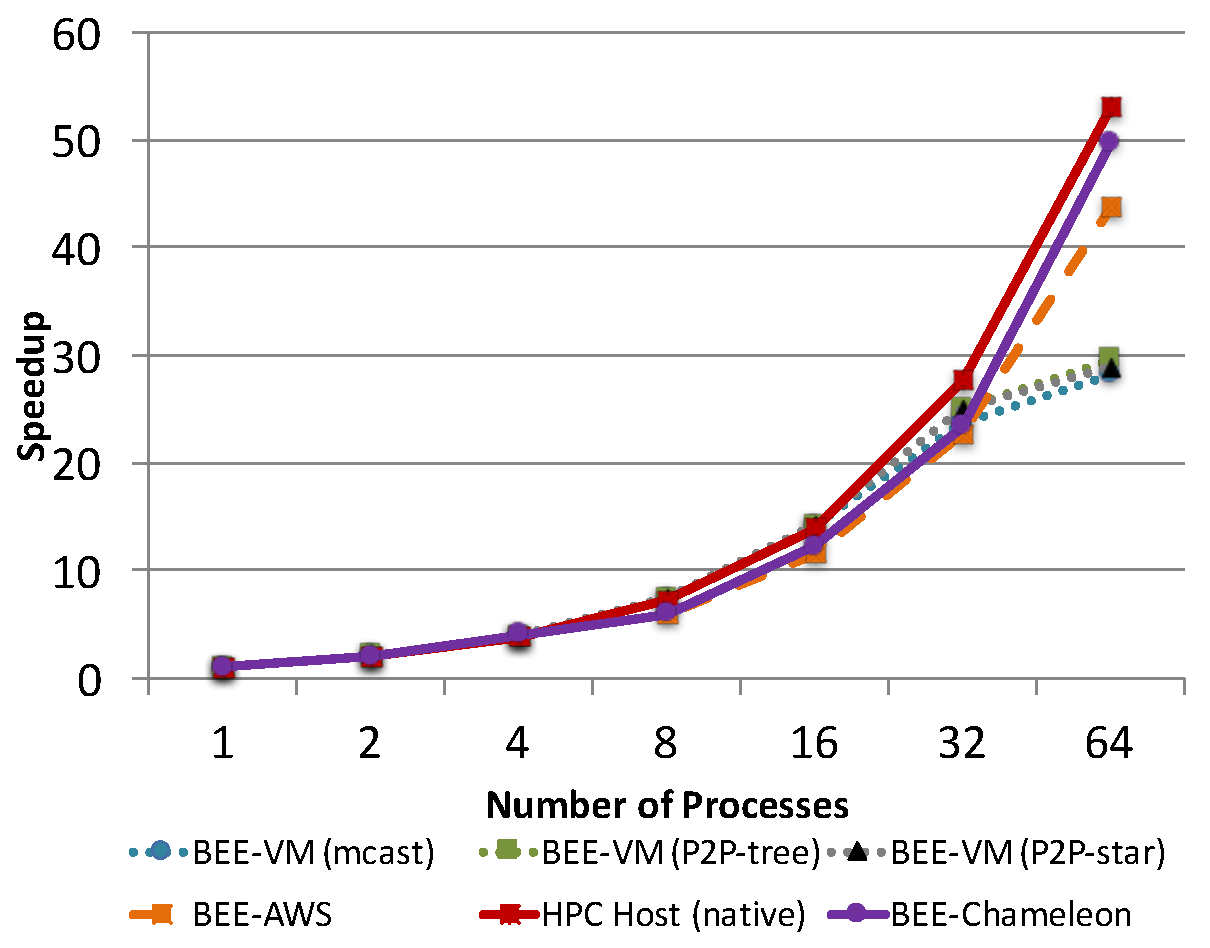
\includegraphics[width=0.5\textwidth]{figures/vpic-test.pdf}
    \caption{VPIC scale up test on \texttt{BEE-VM}, \texttt{BEE-AWS}, \texttt{BEE-Chameleon}, and HPC host. Results show that \texttt{BEE-AWS} and \texttt{BEE-Chameleon} scales similar to HPC native. \texttt{BEE-VM} also scales well under 64 processes, but with lower speedup.}
    \label{vpic-test}
    %\vspace*{-2em}
\end{figure}

We tested VPIC on different environments using 1 to 64 processes. As shown in \textbf{Fig. \ref{vpic-test}}, \texttt{BEE-AWS} and \texttt{BEE-Chameleon} solution scales similarly to the native host.  Our \texttt{BEE-VM} solutions (BEE-mcast, BEE-P2P-tree, and BEE-P2P-star) also scale well from 1 to 64 processes. Among all three network configurations, the tree-shaped connection using P2P sockets works the best. Since in VPIC, one-to-one process communication is much more frequent than all-to-all broadcast, tree-shaped connection can greatly mitigate the hot spot problem under this kind of communication pattern, as discussed before. Depending on the communication pattern in different applications, they may work best with different network designs. Due to the overhead of virtualized network, communication intensive applications, such as VPIC, scale up slower on \texttt{BEE-VM} than on native HPC hosts beyond 64 processes. We will continue to optimize the network performance (e.g., vNIC configuration, connection styles, topology, etc.).

\begin{comment}
\section{BEE in Workflow}
%\jchen{explain how we can integrate workflow logic in to \texttt{BEE}}
By encapsulating the computation provided by HPC (through \texttt{BEE-VM}) or cloud computing systems into containers and separating computation (the container) from state (the data mounts) workflows can be easily composed. Containers are treated as modules that can be easily assembled to form a large workflow system as needed. This enables users to easily build their workflow logic into \texttt{BEE}. Once a user has set the workflow logic,  \texttt{BEE} can deploy and manage user application according to the logic. For example, as shown in \textbf{Figure \ref{workflow}}, when a user wants to a series of pipelined simulations, the user needs to manually configure and start each simulation one by one and also needs to handle data transfer for the pipeline logic. If the pipeline consists of many simulations, it can be considerably difficult to manually deploy and debug, especially when different simulations are conducted on different hosts. However, by using \texttt{BEE}, the user only needs to indicate which simulations need to run and which one follow the other, then \texttt{BEE} can deploy simulation applications in orders and setup the pipeline data transfer. The containerized environment also allows the user to change certain parts of workflow logic at runtime as long as it does not interrupt normal execution.
 %For example, during the pipelined simulation, some soft error or bug occurs and causes incorrect final output data. 
 In-situ analysis as a new approach to diagnose the problem by checking out the intermediate resluts between successive simulation can also be containerized and plug into the workflow. Instead of running the filters and moving data to compete for the computation cycles and I/O bandwidth, In-situ visualization tools can be deployed seperately from the computation codes.  \texttt{BEE-VM} `s I/O design faciliates the in-situ analysis by allowing applying different filters even at the same time to process the data for visualization.
 
Continuous Integration(CI) \cite{fowler2006continuous} has been widely used in many HPC application development process. It is used for unit testing, fixing compatibility issues during integration, etc. Many development projects choose to use standard Docker image as output application format. Since \texttt{BEE} takes standard Docker images as input, it can be seamlessly integrated into CI development.
\begin{figure*}[h]
    \centering
    \caption{BEE with Workflow Integration}
    \label{workflow}
    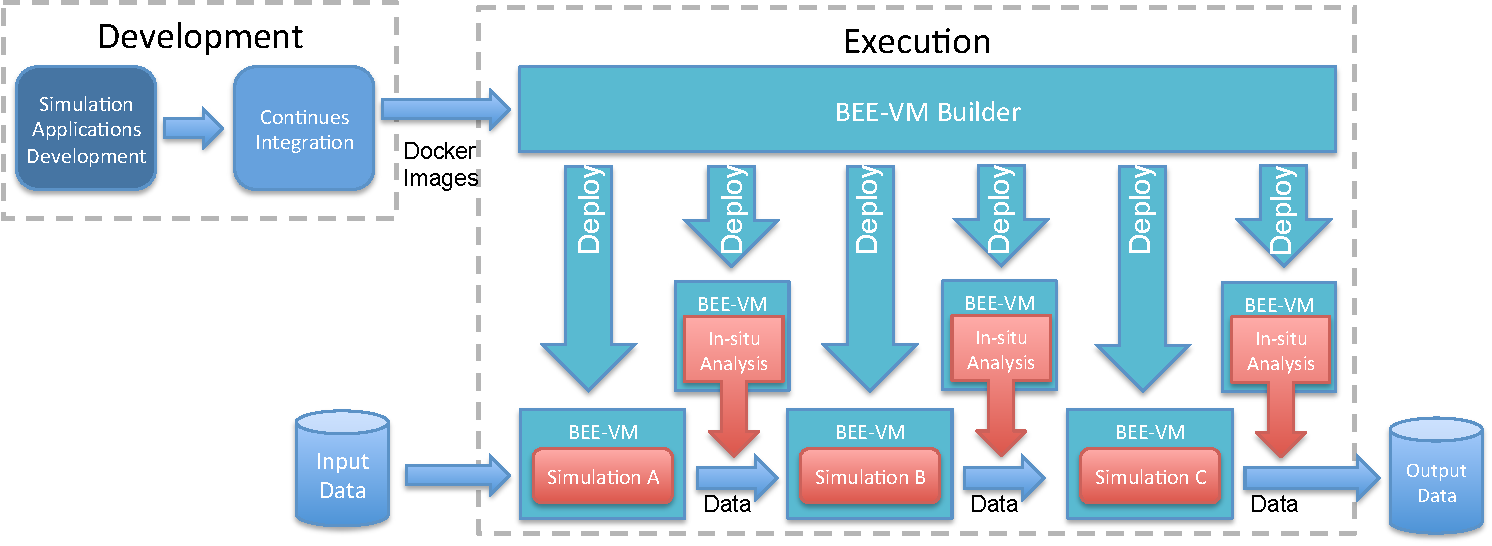
\includegraphics[width=0.75\textwidth]{figures/workflow.pdf}
    \vspace*{-2em}
\end{figure*}

\end{comment}